\NeedRoom{10}

\subsection{Common-Parameter Transfer and Annual Stages}

Comparators use common 2023-CAD cost and energy assumptions, annualizing one week by 365/7. The BC grid factor is a diagnostic transfer, not a local factor. These are method comparisons, not local tariffs, grants or investment forecasts.


\begin{longtable}{@{}L{\dimexpr 0.46000\textwidth-2\tabcolsep\relax}L{\dimexpr 0.27000\textwidth-2\tabcolsep\relax}L{\dimexpr 0.27000\textwidth-2\tabcolsep\relax}@{}}
\caption{Comparator financial and ecological screens under common transferred parameters}\label{tab:source14}\\
\toprule
\textbf{Scenario screen} & \textbf{Chicago} & \textbf{London} \\
\midrule
\endfirsthead
\multicolumn{3}{l}{Table \thetable\ (continued)}\\
\toprule
\textbf{Scenario screen} & \textbf{Chicago} & \textbf{London} \\
\midrule
\endhead
\midrule\multicolumn{3}{r}{Continued on next page}\\\endfoot
\bottomrule\endlastfoot
Annual grid energy (GWh) & 203.6 & 1,267.9 \\
Daytime simultaneous plug sum & 71 & 509 \\
10-year avoided (kt CO$_2$e) & 1,620.7 & 10,497.7 \\
0\% grant NPV (CAD m) & -1.9 & 1,702.9 \\
25\% grant NPV (CAD m) & 260.2 & 2,912.2 \\
50\% grant NPV (CAD m) & 522.3 & 4,121.5 \\
\end{longtable}

\begin{figure}[htbp]\centering

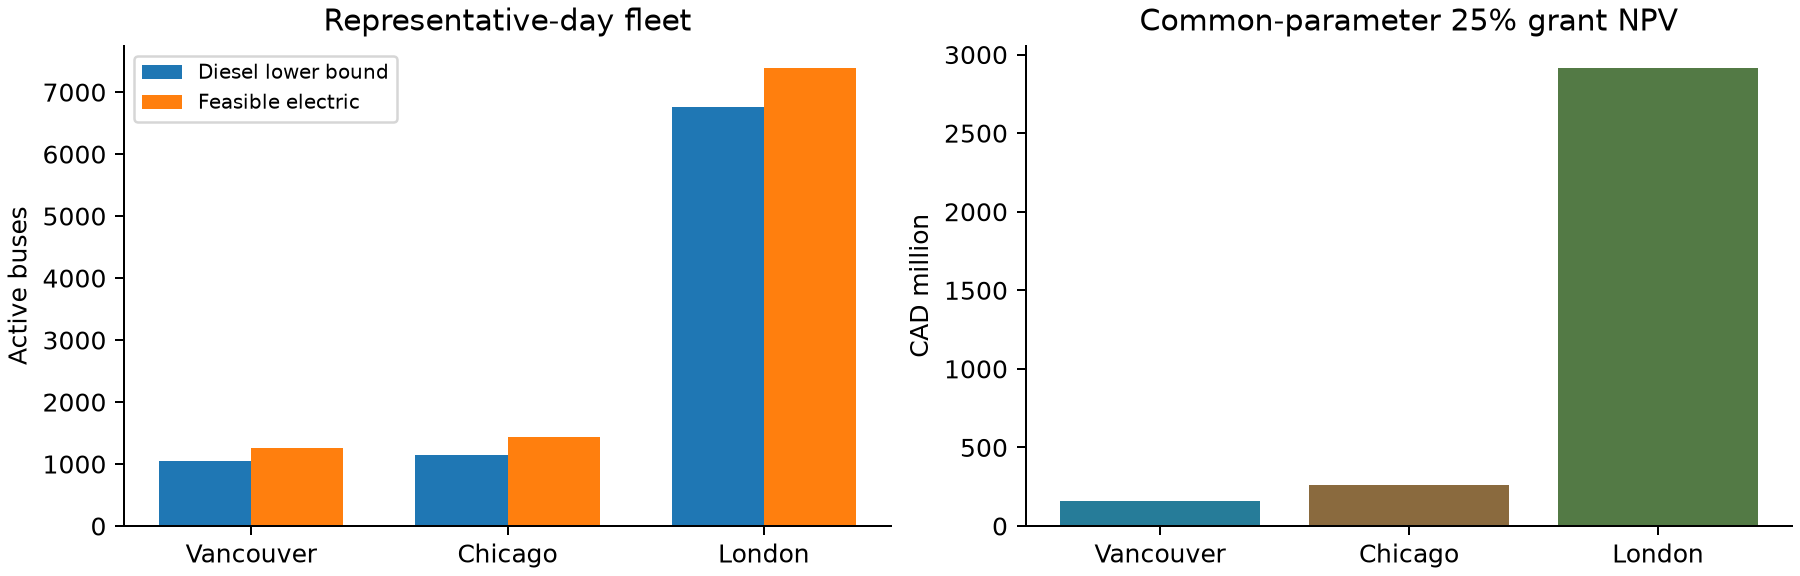
\includegraphics[width=\textwidth,height=0.37\textheight,keepaspectratio]{images/threecity_comparison.png}

\caption{Representative-day diesel/electric fleets and common-parameter 25\% grant NPV.}\label{fig:result5}

\end{figure}

\begin{longtable}{@{}L{\dimexpr 0.11000\textwidth-2\tabcolsep\relax}L{\dimexpr 0.14000\textwidth-2\tabcolsep\relax}L{\dimexpr 0.14000\textwidth-2\tabcolsep\relax}L{\dimexpr 0.15000\textwidth-2\tabcolsep\relax}L{\dimexpr 0.15000\textwidth-2\tabcolsep\relax}L{\dimexpr 0.14000\textwidth-2\tabcolsep\relax}L{\dimexpr 0.17000\textwidth-2\tabcolsep\relax}@{}}
\caption{Comparator annual purchases, residual diesel fleets and gross investment}\label{tab:source15}\\
\toprule
\textbf{Year} & \textbf{CTA new EV} & \textbf{CTA diesel} & \textbf{CTA gross (m)} & \textbf{London new EV} & \textbf{London diesel} & \textbf{London gross (m)} \\
\midrule
\endfirsthead
\multicolumn{7}{l}{Table \thetable\ (continued)}\\
\toprule
\textbf{Year} & \textbf{CTA new EV} & \textbf{CTA diesel} & \textbf{CTA gross (m)} & \textbf{London new EV} & \textbf{London diesel} & \textbf{London gross (m)} \\
\midrule
\endhead
\midrule\multicolumn{7}{r}{Continued on next page}\\\endfoot
\bottomrule\endlastfoot
2024 & 122 & 1056 & 309.4 & 995 & 5879 & 2,066.8 \\
2025 & 195 & 908 & 233.4 & 1039 & 4929 & 1,243.8 \\
2026 & 173 & 779 & 206.6 & 998 & 3995 & 1,191.9 \\
2027 & 148 & 670 & 176.3 & 1068 & 3000 & 1,272.5 \\
2028 & 177 & 532 & 210.4 & 1038 & 2004 & 1,234.0 \\
2029 & 176 & 393 & 208.8 & 890 & 1169 & 1,055.8 \\
2030 & 157 & 284 & 185.9 & 661 & 572 & 782.5 \\
2031 & 191 & 117 & 225.6 & 494 & 241 & 583.6 \\
2032 & 50 & 63 & 68.2 & 122 & 135 & 219.6 \\
2033 & 47 & 0 & 69.7 & 96 & 0 & 189.7 \\
\end{longtable}

Stages rerun electric and residual-diesel scheduling, and stock never decreases. All grant and funding columns, route lists and duties are supplied separately. All modeled fixed-time obligations become electric by 2033.


These are required budgets, not solutions under known annual spending caps. Initial power and site capacity, vehicle ages, construction dates, zero-source electricity and local prices remain unverified.

